% =====================================================================
%  Presentación del proyecto TEL252 — Firmas digitales basadas en hash
%  Compilar: latexmk -pdf main.tex   (dentro de Proyecto/presentacion/)
%  Formato (Lección 0, ítem 4): máx. 15 min = intro 3–5' + video 5'
%  + conclusiones y preguntas en máx. 7'. Las figuras salen del informe.
%  \pend{...} = dato que falta (en rojo); se apaga con \borradorfalse.
% =====================================================================
\documentclass[aspectratio=169,11pt]{beamer}
\usepackage[utf8]{inputenc}
\usepackage[spanish,es-tabla]{babel}
\usepackage{amsmath,amssymb}
\usepackage{graphicx}
\usepackage{booktabs}
\usepackage{tikz}
\usetikzlibrary{positioning,arrows.meta,calc}

\usetheme{default}
\usecolortheme{seahorse}
\setbeamertemplate{navigation symbols}{}
\setbeamertemplate{footline}[frame number]
\setbeamertemplate{itemize items}[circle]

\graphicspath{{../informe-tel252/figuras/}}

\newif\ifborrador \borradortrue   % <- cambiar a \borradorfalse para la presentación
\newcommand{\pend}[1]{\ifborrador\textcolor{red}{\textbf{[#1]}}\fi}
\newcommand{\ok}{\textcolor{green!50!black}{\checkmark}}
\definecolor{azul}{HTML}{4C72B0}
\definecolor{rojo}{HTML}{C44E52}

\title{Firmas basadas en hash vs.\ ECDSA}
\subtitle{El costo de resistir al cuántico}
\author{Equipo Hashquantum (grupo 12)\\[2pt]
  \small Josué Leiva \;·\; Sebastián Moya \;·\; Cristian Pizarro \;·\; Bastián Reyes}
\institute{TEL252 Criptografía y Seguridad de la Información\\Universidad Técnica Federico Santa María}
\date{}

\begin{document}

% ---------- 0:00 ----------
\begin{frame}
  \titlepage
\end{frame}

% ---------- 0:15 Problema ----------
\begin{frame}{Problema: las firmas actuales no resisten un computador cuántico}
  \begin{itemize}
    \item RSA, DSA y ECDSA se basan en factorizar enteros y en el logaritmo discreto.
    \item El algoritmo de \textbf{Shor} resuelve ambos en tiempo polinomial: alargar las claves no basta.
    \item El NIST (IR 8547) propone \textbf{dejar de permitir} ECDSA y RSA después de \textbf{2035}.
  \end{itemize}
  \vspace{0.8em}
  \begin{block}{Alternativa: firmas basadas en hash}
    Su seguridad depende \textbf{solo} de la función hash (SHA-256). Grover la debilita de forma
    cuadrática: una preimagen sigue costando $\sim2^{128}$ operaciones.
    Estandarizadas en SP 800-208 (XMSS, LMS) y FIPS 205 (SLH-DSA).
  \end{block}
  \vspace{0.4em}
  \centering\textbf{¿Cuánto cuesta esa seguridad en tamaño y en tiempo?}
\end{frame}

% ---------- 1:00 WOTS ----------
\begin{frame}{WOTS: firmar dígitos con cadenas de hash}
  \centering
  \begin{tikzpicture}[node distance=1.15cm, every node/.style={font=\small},
      n/.style={draw, rounded corners, minimum width=1.25cm, minimum height=0.65cm, fill=white},
      a/.style={-{Stealth}, thick}]
    \node[n, fill=gray!15] (x) {$x$};
    \node[n, right=of x] (h1) {$H(x)$};
    \node[right=0.5cm of h1] (dots) {$\cdots$};
    \node[n, right=0.5cm of dots, fill=azul!25] (hd) {$H^{d}(x)$};
    \node[right=0.5cm of hd] (dots2) {$\cdots$};
    \node[n, right=0.5cm of dots2, fill=green!20] (pk) {$H^{w-1}(x)$};
    \draw[a] (x) -- (h1); \draw[a] (h1) -- (dots); \draw[a] (dots) -- (hd);
    \draw[a] (hd) -- (dots2); \draw[a] (dots2) -- (pk);
    \node[below=0.15cm of x] {\scriptsize secreto};
    \node[below=0.15cm of hd] {\scriptsize firma del dígito $d$};
    \node[below=0.15cm of pk] {\scriptsize clave pública};
    \draw[thick, rojo, -{Stealth}] ($(hd.north)+(0,0.1)$) to[bend left=25]
      node[above] {\scriptsize verificar: $w-1-d$ hashes más} ($(pk.north)+(0,0.1)$);
  \end{tikzpicture}
  \vspace{0.6em}
  \begin{itemize}
    \item El resumen $H(m)$ se parte en $\ell_1$ dígitos en base $w$; una suma de control ($\ell_2$ dígitos)
          impide avanzar en las cadenas.
    \item $|\sigma_{\mathrm{WOTS}}| = 32\,\ell$ bytes, con $\ell = \ell_1+\ell_2$: \;
          $w=4 \to \ell=133$, \; $w=16 \to 67$, \; $w=256 \to 34$.
    \item \textbf{Compromiso:} más $w$ = menos cadenas (firma chica), pero cadenas más largas (más cómputo).
    \item Es de \textbf{un solo uso}: firmar dos veces con la misma clave filtra secretos.
  \end{itemize}
\end{frame}

% ---------- 2:00 Merkle ----------
\begin{frame}{Árbol de Merkle: muchas firmas con una sola clave pública}
  \begin{columns}[c]
    \column{0.5\textwidth}
    \centering
    \begin{tikzpicture}[every node/.style={font=\scriptsize},
        n/.style={draw, circle, minimum size=0.55cm, inner sep=0pt, fill=white},
        l/.style={draw, minimum size=0.5cm, inner sep=1pt, fill=gray!10},
        level distance=0.95cm]
      \node[n, fill=green!25] (r) at (0,0) {raíz};
      \node[n] (a) at (-1.6,-1) {};       \node[n, fill=orange!35] (b) at (1.6,-1) {};
      \node[n, fill=orange!35] (c) at (-2.4,-2) {}; \node[n] (d) at (-0.8,-2) {};
      \foreach \i/\x in {0/-2.8,1/-2.0,2/-1.2,3/-0.4} {\node[l] (L\i) at (\x,-3) {$\mathrm{pk}_{\i}$};}
      \node[l, fill=azul!30] at (L2) {$\mathrm{pk}_{2}$};
      \node at (1.6,-3) {$\cdots\ \mathrm{pk}_{15}$};
      \draw (r)--(a) (r)--(b) (a)--(c) (a)--(d) (c)--(L0) (c)--(L1) (d)--(L2) (d)--(L3);
      \node[l, fill=orange!35] at (-0.4,-3) {$\mathrm{pk}_{3}$};
      \draw[very thick, azul] (L2)--(d)--(a)--(r);
    \end{tikzpicture}

    \scriptsize\textcolor{azul}{azul}: camino que recalcula el verificador;
    \textcolor{orange!80!black}{naranjo}: hermanos incluidos en la firma
    \column{0.5\textwidth}
    \begin{itemize}
      \item $2^h$ claves WOTS; cada hoja es el hash de una clave pública.
      \item La \textbf{raíz} (32 B) es la clave pública global.
      \item Firma $i$ = firma WOTS + su clave pública + $h$ hermanos + índice:
            \[|\sigma| = |\sigma_{\mathrm{WOTS}}| + 32 + 32h + 4\ \mathrm{B}\]
      \item \textbf{Con estado:} el firmante nunca debe repetir un índice; con $h=4$ son 16 firmas.
    \end{itemize}
  \end{columns}
\end{frame}

% ---------- 3:00 Hipótesis ----------
\begin{frame}{Hipótesis y objetivos}
  \begin{block}{Hipótesis}
    Un árbol de Merkle ($h=4$) con WOTS ($w=16$), en Python puro, verifica en
    \textbf{menos de 5 veces} el tiempo de ECDSA P-256 (en C), con una firma
    \textbf{30 a 40 veces} más grande. Pasar de $w=4$ a $w=256$ reduce la firma a
    \textbf{menos de un tercio} y multiplica por \textbf{más de 10} los tiempos.
  \end{block}
  \textbf{Objetivo general:} medir el costo en tamaño y tiempo de una firma basada en hash
  implementada desde cero, frente a ECDSA P-256.
  \begin{itemize}
    \item Implementar Lamport, WOTS y Merkle con SHA-256, y validarlos.
    \item Medir tamaños y tiempos para $w\in\{4,16,256\}$.
    \item Demostrar con un ataque que reutilizar una clave de un solo uso permite falsificar.
  \end{itemize}
\end{frame}

% ---------- 3:45 Metodología ----------
\begin{frame}{Metodología}
  \begin{columns}[T]
    \column{0.55\textwidth}
    \begin{enumerate}
      \item \textbf{Implementación:} Python 3.13 + \texttt{hashlib}; interfaz común
            \texttt{keygen}/\texttt{sign}/\texttt{verify}. ECDSA desde \texttt{cryptography}.
      \item \textbf{Validación:} firma válida acepta; mensaje alterado y otra clave rechazan.
      \item \textbf{Medición:} $N = 10\,000$ repeticiones, 10 de calentamiento,
            \texttt{perf\_counter}; media $\pm$ desviación estándar.
      \item \textbf{Análisis:} cada parte de la hipótesis contra su umbral, y tiempo medido contra
            número teórico de hashes.
    \end{enumerate}
    \column{0.42\textwidth}
    \begin{block}{Variables}
      \small
      \textbf{Independiente:} $w$\\
      \textbf{Dependientes:} tamaños; tiempo de claves, firma y verificación\\
      \textbf{Controladas:} SHA-256, $h=4$, $N$, versión de Python y equipo
      (Ryzen 5 5600GT, 14 GiB, Ubuntu 26.04)
    \end{block}
  \end{columns}
\end{frame}

% ---------- 4:30 Video ----------
\begin{frame}{Prueba de concepto (video, 5 min)}
  \centering
  \Large\url{https://youtu.be/VIDEO} \pend{link}\\[1em]
  \normalsize
  \begin{columns}[T]
    \column{0.32\textwidth}
    \begin{block}{1. Validación}
      \small Cada esquema firma, verifica y rechaza un mensaje alterado.
    \end{block}
    \column{0.32\textwidth}
    \begin{block}{2. Ataque a Lamport}
      \small $k=6$ firmas con la misma clave: $\sim2^{8}$ intentos para falsificar
      «Transferir \$1000 a Mallory».
    \end{block}
    \column{0.32\textwidth}
    \begin{block}{3. Estado en Merkle}
      \small 16 firmas válidas; la firma 17 se rechaza (claves agotadas).
    \end{block}
  \end{columns}
\end{frame}

% ---------- 9:30 Resultados ----------
\begin{frame}{Resultados ($N=10\,000$)}
  \begin{columns}[c,onlytextwidth]
    \column{0.37\textwidth}
    \centering
    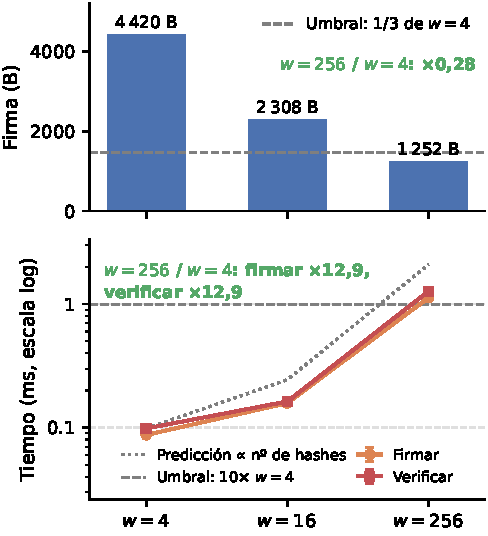
\includegraphics[width=\linewidth,height=0.78\textheight,keepaspectratio]{tamano_tiempo_w.pdf}\\
    \scriptsize (a) efecto de $w$
    \column{0.37\textwidth}
    \centering
    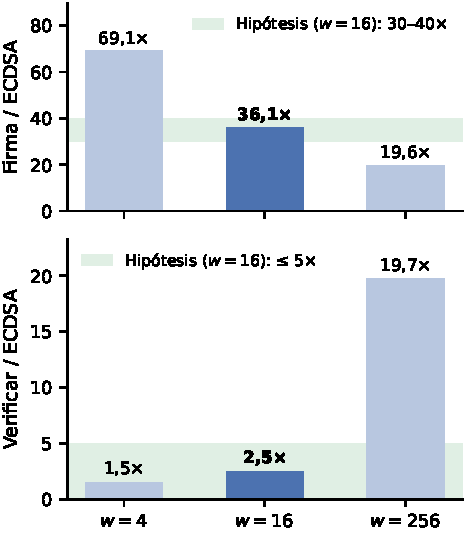
\includegraphics[width=\linewidth,height=0.78\textheight,keepaspectratio]{comparacion_ecdsa.pdf}\\
    \scriptsize (b) frente a ECDSA
    \column{0.24\textwidth}
    \small
    \textbf{Merkle, $w=16$}
    \begin{itemize}
      \item Firma: 2\,308 B\\(ECDSA: 64 B)
      \item Verificar: 0,163 ms\\(ECDSA: 0,064 ms)
      \item Generar el árbol: 5,3 ms
    \end{itemize}
  \end{columns}
\end{frame}

% ---------- 10:15 Contraste ----------
\begin{frame}{Contraste con la hipótesis: se cumplen las 4 partes}
  \centering
  \begin{tabular}{llll}
    \toprule
    Parte de la hipótesis & Umbral & Medido & \\
    \midrule
    Verificar, $w=16$ / ECDSA       & $< 5\times$        & $2{,}5\times$  & \ok \\
    Firma, $w=16$ / ECDSA           & $30$–$40\times$    & $36{,}1\times$ & \ok \\
    Firma, $w=256$ / $w=4$          & $< 1/3$            & $0{,}28$       & \ok \\
    Firmar y verificar, $w=256$ / $w=4$ & $> 10\times$   & $12{,}9\times$ & \ok \\
    \bottomrule
  \end{tabular}
  \vspace{1em}
  \begin{itemize}
    \item \textbf{Predicción vs medición:} los hashes crecen $21{,}2\times$ (204,5 $\to$ 4\,340), pero el
          tiempo solo $12{,}9\times$: el intérprete agrega un costo fijo por cadena que pesa más con $w=4$.
    \item ECDSA corre en C y Merkle en Python puro: la comparación \textbf{favorece a ECDSA}, así que
          $2{,}5\times$ es conservador. Dispersión: 2–5\,\% de la media.
  \end{itemize}
\end{frame}

% ---------- 11:00 Conclusiones ----------
\begin{frame}{Conclusiones}
  \begin{itemize}
    \item Una firma basada en hash es viable en tiempo: verificar cuesta solo $2{,}5\times$ ECDSA,
          incluso en Python puro.
    \item El precio real es el \textbf{tamaño}: $36\times$ más bytes con $w=16$.
    \item $w$ es la perilla del compromiso: $w=256$ achica la firma a 1\,252 B, pero verifica
          $\sim$13 veces más lento.
    \item El \textbf{estado} es crítico: reutilizar una clave de un solo uso permite falsificar
          \pend{resultado del ataque a Lamport}, y Merkle debe rechazar índices agotados.
  \end{itemize}
  \vspace{0.6em}
  \textbf{Trabajo futuro:} W-OTS+, SLH-DSA (sin estado) e implementación en C.
\end{frame}

% ---------- 11:45 Cierre ----------
\begin{frame}
  \centering
  {\Large ¡Gracias! ¿Preguntas?}\\[1.5em]
  \scriptsize Código: \url{https://github.com/josue-fourier/Tareas-TEL252-Crypto-2026-2/tree/main/Proyecto/codigo}
\end{frame}

\begin{frame}{Referencias}
  \scriptsize
  \begin{itemize}
    \item Merkle, R. C. (1989). A certified digital signature. \emph{CRYPTO '89}.
    \item Shor, P. W. (1994). Algorithms for quantum computation. \emph{FOCS}.
    \item Grover, L. K. (1996). A fast quantum mechanical algorithm for database search. \emph{STOC}.
    \item NIST (2020). \emph{SP 800-208: Recommendation for stateful hash-based signature schemes}.
    \item NIST (2024). \emph{FIPS 205: Stateless hash-based digital signature standard}.
    \item NIST (2024). \emph{IR 8547 (borrador): Transition to post-quantum cryptography standards}.
  \end{itemize}
\end{frame}

% ---------- Respaldo (para preguntas) ----------
\appendix
\begin{frame}{Respaldo: tiempos por operación (ms, media $\pm$ desv. est.)}
  \centering
  \small
  \begin{tabular}{lrrrr}
    \toprule
    Esquema & Generar claves & Firmar & Verificar & Verif./ECDSA \\
    \midrule
    Merkle $w=4$   & 3,415 $\pm$ 0,065  & 0,087 $\pm$ 0,005 & 0,098 $\pm$ 0,004 & 1,5 \\
    Merkle $w=16$  & 5,251 $\pm$ 0,093  & 0,158 $\pm$ 0,006 & 0,163 $\pm$ 0,008 & 2,5 \\
    Merkle $w=256$ & 38,168 $\pm$ 0,631 & 1,124 $\pm$ 0,029 & 1,270 $\pm$ 0,033 & 19,7 \\
    ECDSA P-256    & 0,014 $\pm$ 0,001  & 0,032 $\pm$ 0,002 & 0,064 $\pm$ 0,005 & 1 \\
    \bottomrule
  \end{tabular}
  \vspace{1em}

  \small Tamaños de firma: Merkle 4\,420 / 2\,308 / 1\,252 B ($w=4/16/256$); ECDSA 64 B ($r\Vert s$).
\end{frame}

\end{document}
